\documentclass[a4paper]{article}

\usepackage[utf8]{inputenc}
\usepackage[portuges]{babel}
\usepackage{indentfirst}
\usepackage{graphicx}
\usepackage{float}

\title{Projeto de Laboratórios de Informática 3\\Grupo 21}
\author{Diogo Braga A82547 \and João Silva A82005 \and Ricardo Caçador A81064}
\date{\today}

\begin{document}

\maketitle

\begin{abstract}
Este documento apresenta o projeto de Laboratórios de Informática
3 (LI3), do curso de Engenharia Informática da Universidade
do Minho.

O projeto baseia-se na criação de um sistema de análise de ficheiros 
XML que possuem informações do Stack Overflow, um website de perguntas
e respostas sobre programação de computadores.

\end{abstract}

\tableofcontents
\listoffigures

\section{Introdução}
\label{sec:intro}

Este trabalho tem por base o parse de elementos de ficheiros XML
relacionados com a informação do website Stack Overflow, de forma
a seguidamente responder a uma série de questões relacionadas com
posts, utilizadores e tags do mesmo website. Aliado a tal está o desafio
de procurar sempre o melhor algoritmo de resolução das queries, de 
forma a tornar o código mais eficiente e o mais rápido possível.

A Secção ~\ref{sec:estruturas} apresenta as estruturas de dados utilizadas 
no projeto, a Secção~\ref{sec:modularidade} aborda a modularidade, 
a Secção ~\ref{sec:encapsulamento} aborda o encapsulamento, a 
Secção ~\ref{sec:abstracao_de_dados} aborda a abstração de dados e a 
Secção~\ref{sec:estrategias} indica as estratégias usadas para resolver 
as questões apresentadas. O relatório termina com conclusões na
Secção~\ref{sec:conclusao}, onde é também apresentada uma análise
crítica dos resultados obtidos.

\section{Estruturas de Dados}
\label{sec:estruturas}

Este trabalho tem por base uma estrutura principal denominada \textbf{TCD}, 
sendo que depois é utilizada esta mesma mas com abstração de dados, a 
\textbf{TAD}.

Esta estrutura possui:
\begin{itemize}
	\item Uma \textbf{struct utilizador} que contêm os atributos do utilizador
e está definida como \textit{\textbf{GHashTable*}};
	\item Uma \textbf{struct posts} que contêm os atributos de um post e
está definida como \textit{\textbf{GHashTable*}};
	\item Uma \textbf{struct date\_posts} que contêm os atributos de um post
está definida como \textit{\textbf{GList*}}, sendo esta ordenada por data;
	\item Uma \textbf{struct tags} que contêm os atributos de uma tag e
está definida como \textit{\textbf{GHashTable*}}.
\end{itemize}

\begin{figure}[H]
\centering
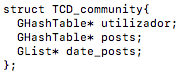
\includegraphics[scale=0.70]{image_tcd}
\caption{Estrutura \textit{TCD}}
\label{img:tcd}
\end{figure}

\begin{figure}[H]
\centering
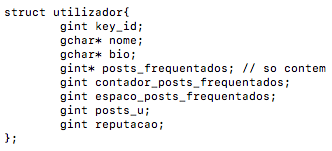
\includegraphics[scale=0.70]{image_utilizador}
\caption{Estrutura \textit{Utilizador}}
\label{img:utilizador}
\end{figure}

\begin{figure}[H]
\centering
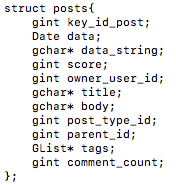
\includegraphics[scale=0.70]{image_posts}
\caption{Estrutura \textit{Posts}}
\label{img:posts}
\end{figure}

\begin{figure}[H]
\centering
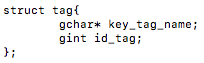
\includegraphics[scale=0.70]{image_tag}
\caption{Estrutura \textit{Tag}}
\label{img:tag}
\end{figure}

\newpage

\section{Modularidade}
\label{sec:modularidade}

Modularidade, por definição, é a divisão do código fonte em unidades 
separadas coerentes. É algo que temos em conta no nosso projeto,
existindo, por base, o ficheiro \textbf{main.c}, e depois todos os
ficheiros individuais relacionados com as \textbf{estruturas de dados}
usadas e as \textbf{queries} propostas. Estes possuem os ficheiros 
\textbf{.c} que contêm o código fonte e os \textbf{.h/header files} que
definem o que é invocável do exterior.

Modularidade torna-se portanto fundamental para lidar com a complexidade
do código, de tal forma que o código dos programas deve ser dividido por
unidades modulares pequenas e autônomas, devendo-se ter em especial atenção
a criação dos módulos que representam \textbf{abstração de dados}.

\section{Encapsulamento}
\label{sec:encapsulamento}

Encapsulamento baseia-se na garantia de \textbf{protecção} e 
\textbf{acessos controlados aos dados}. É mais um aspeto que temos em 
conta no nosso projeto de forma a que exista uma divisão entre as operações 
que são públicas e aquelas que são internas ao módulo. Estas são privadas e,
portanto, são apenas acessíveis do exterior atráves das funções
disponibilizadas na \textbf{API}. Algo vísivel na figura 
~\ref{img:encapsulamento_posts}, neste caso abordando as \textbf{tags}.

Desta forma um tipo de dados permite ter várias instanciações,
visto que os módulos das estruturas e das queries se tornam mais genéricos.

\begin{figure}[H]
\centering
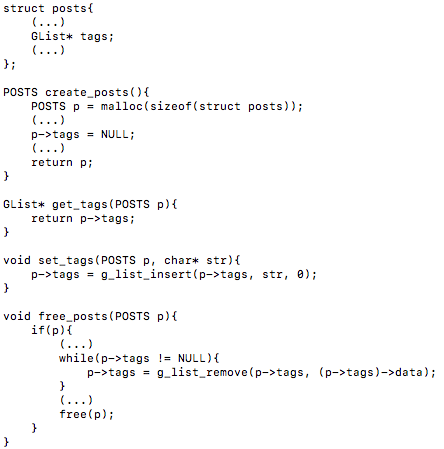
\includegraphics[scale=0.60]{image_exemplo_encapsulamento}
\caption{Exemplo Encapsulamento \textit{Tags}}
\label{img:encapsulamento_posts}
\end{figure}

\section{Abstração de Dados}
\label{sec:abstracao_de_dados}

A declaração abstrata duma estrutura esconde dos utilizadores do módulo a
implementação concreta, não tendo desta forma acesso à implementação
da mesma. Por isso mesmo, previamente, temos a declaração abstrata da 
estrutura \textbf{utilizador}, denominada de \textbf{UTILIZADOR}, no
\textit{header file}, como mostra o exemplo ~\ref{img:declaracao_utilizador}.

\begin{figure}[H]
\centering
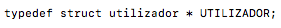
\includegraphics[scale=0.70]{image_declaracao_utilizador}
\caption{Exemplo Declaração Abstrata \textit{utilizador}}
\label{img:declaracao_utilizador}
\end{figure}

\section{Estratégias das Interrogações}
\label{sec:estrategias}

\subsection{Init}

Função que cria a \textbf{TCD\_community}. Por consequência, inicializa
as estruturas relacionadas a essa mesma struct, alocando memória e usando
a função da \textit{glib}, \textbf{g\_hash\_table\_new}.

\subsection{Load}

Função que realiza o parse de todos os ficheiros necessários à realização
do trabalho. Após receber um \textbf{dump\_path} para os ficheiros XML,
caso não existam falhas na estrutura XML são realizadas três funções:
o \textbf{getReferenceUser}, o \textbf{getReferencePosts} e o
\textbf{getReferenceTags}.

A primeira realiza todo o parse relacionado com os \textbf{utilizadores}, 
como por exemplo o \textbf{id} ou a \textbf{reputação}. De seguida são 
colocados na estrutura todos estes elementos através da função
\textbf{set\_utilizador}.

A segunda realiza todo o parse relacionado com os \textbf{posts}, 
como por exemplo o \textbf{id\_post} ou o \textbf{post\_type\_id}. 
De seguida são colocados na estrutura todos estes elementos através da 
função \textbf{set\_posts}.

A terceira realiza todo o parse relacionado com as \textbf{tags}, 
como por exemplo o \textbf{id\_tag} ou o \textbf{tag\_name}. 
De seguida são colocados na estrutura todos estes elementos através da 
função \textbf{set\_tag}.

\subsection{Query 1}

Dado o identificador de um post, a função retorna o título do post 
e o nome de utilizador do autor. Se o post for uma resposta, a função
retorna o título e o id do utilizador da pergunta correspondente.

Nesta questão, sendo o valor do \textbf{id} igual ao da \textbf{key} 
da tabela de hash, recorremos à função da \textit{glib},
\textbf{g\_hash\_table\_lookup} que dado uma \textbf{key},
retorna o \textbf{value} associado. Caso nada seja encontrado,
é retornado NULL.

Tendo agora todos os valores referentes ao \textbf{post}, caso este
seja uma pergunta, é atríbuido à primeira coordenada o \textbf{title}
do post e à segunda o \textbf{nome} de quem realizou a questão.
Encontramos o \textbf{nome} do autor da questão invocando o parâmetro
\textbf{owner\_user\_id} na mesma função \textbf{lookup} utilizada 
anteriormente, passando agora a ser esse o \textbf{key/id} associado.

Caso seja uma resposta, o primeiro parâmetro é calculado usando a mesma 
função \textbf{g\_hash\_table\_lookup}, mas agora com o 
parâmetro \textbf{parent\_id}, que numa resposta retorna o \textbf{id} 
da pergunta ao qual esta respondeu. O segundo parâmetro é igualmente
calculado como se fosse uma pergunta, mudando apenas o novo 
\textbf{value} associado.

\subsection{Query 2}

Pretendemos obter o top N utilizadores com maior número de posts de 
sempre. Para isto, são considerados tanto perguntas quanto respostas 
dadas pelo respectivo utilizador.

Nesta questão, utilizamos uma \textit{\textbf{GList*}} para armazenar 
os \textbf{values} de cada \textbf{utilizador}, sendo isto realizado
pela função da \textit{glib}, \textbf{g\_hash\_table\_get\_values}.

Depois esta lista é ordenada por número de posts (de cada utilizador)
em ordem decrescente através da função da \textit{glib}, 
\textbf{g\_list\_sort}, que usa uma função de comparação 
\textbf{compara\_posts\_u}, que tem em conta o parâmetro
\textbf{posts\_u} da estrutura.

De seguida, fazemos a filtração para o \textbf{set\_list} do 
\textbf{id} de cada utilizador.

\subsection{Query 3}

Dado um intervalo de tempo arbitrário, obtemos o número total de posts 
(identificando perguntas e respostas separadamente) neste período.

Nesta questão, utilizamos uma \textit{\textbf{GList*}} para armazenar 
os \textbf{posts} ordenados por data que se encontram na estrutura 
\textbf{date\_posts}, para de seguida percorrer estes mesmos posts.

Enquanto isso, verificamos se a \textbf{data} do post se encontra entre 
os limites referenciados pela query, através da função \textbf{difDatas},
e caso seja uma pergunta, é incrementada a primeira coordenada do par,
caso contrário é uma resposta, e é incrementada a segunda coordenada.

\subsection{Query 4}

Dado um intervalo de tempo arbitrário, retornamos todas as perguntas 
contendo uma determinada tag. O retorno da função é uma lista com os IDs 
das perguntas ordenadas em cronologia inversa.

Nesta questão, utilizamos uma \textit{\textbf{GList*}} para armazenar 
os \textbf{posts} ordenados por data que se encontram na estrutura 
\textbf{date\_posts}.

Enquanto isso, verificamos se a \textbf{data} do post se encontra entre 
os limites referenciados pela query, através da função \textbf{difDatas},
e se é uma pergunta. Nos posts em que os dois parâmetros são cumpridos,
colocamos as tags desses mesmos posts uma nova \textit{GList*}
usando a função \textbf{get\_tags}. Verificamos se a \textbf{tag} passada 
como parâmetro pertence à lista anterior usando a função \textbf{strcmp},
e caso pertença é inserida no início duma \textit{GList*} \textbf{res} 
que vai conter os resultados finais, através da função 
\textbf{g\_list\_insert}.

De seguida, ordenamos a lista \textbf{res} por data através da função
\textbf{g\_list\_sort}, de modo a depois poder retornar os \textbf{id's}
em questão.

\subsection{Query 5}

Dado um ID de utilizador, devolvemos a informação do seu perfil (short 
bio) e os IDs dos seus 10 últimos posts (perguntas ou respostas), 
ordenados por cronologia inversa.

Nesta questão, recorremos à função da \textit{glib}, 
\textbf{g\_hash\_table\_lookup}, para termos o \textbf{value} 
associado ao \textbf{id} do utilizador. Desta forma, retornamos a 
\textbf{bio} do utilizador.

Retornamos os últimos 10 posts acedendo à estrutura que tem os posts
ordenados por data e, começando no último elemento da \textit{
\textbf{GList*}}, vamos percorrendo a lista para trás. Caso o 
\textbf{owner\_user\_id} seja o requerido adicionamos o \textbf{id} 
do post à lista a retornar.

\subsection{Query 6}

Dado um intervalo de tempo arbitrário, devolver os IDs das N respostas 
com mais votos, em ordem decrescente do número de votos.

Nesta questão, recorremos à estrutura \textbf{date\_posts} que possuí 
as datas ordenadas. Caso o \textbf{post} seja uma pergunta e
se encontre entre as datas requeridas na query, é inserida numa nova
\textit{\textbf{GList*}} \textbf{glvotes} criada para armazenar os 
valores necessários para a resposta final.

Depois esta lista é ordenada por votos em ordem decrescente através da 
função da \textit{glib}, \textbf{g\_list\_sort}, que usa uma função de 
comparação \textbf{compara\_score}, que tem em conta o \textbf{score}
da estrutura. Finalmente acedemos ao \textbf{id\_post} relacionado, 
através dos dados respetivos da lista \textbf{glvotes}.

\subsection{Query 7}

Dado um intervalo de tempo arbitrário, devolver os IDs das N perguntas 
com mais respostas, em ordem decrescente do número de votos.

Nesta questão, recorremos à estrutura \textbf{date\_posts} que possuí 
as datas ordenadas. Caso o \textbf{post} seja uma resposta e
se encontre entre as datas requeridas na query, é inserida numa nova
\textit{\textbf{GList*}} \textbf{glanswers} criada para armazenar os 
valores necessários para a resposta final.

Depois esta lista é ordenada por número de respostas em ordem decrescente
através da função da \textit{glib}, \textbf{g\_list\_sort}, que usa uma 
função de comparação \textbf{compara\_answer}, que tem em conta o 
\textbf{answer\_count} da estrutura. Finalmente acedemos ao \textbf{id\_post}
relacionado, através dos dados respetivos da lista \textbf{glanswers}.

\subsection{Query 8}

Dado uma palavra, devolver uma lista com os IDs de N perguntas
cujos títulos a contenham, ordenados por cronologia inversa.

Nesta questão, recorremos à estrutura \textbf{date\_posts} que possuí 
as datas ordenadas. A lista dos posts é iterada do fim para o início
de modo a ir em conta da cronologia inversa. Caso o \textbf{post} seja 
uma pergunta, e, usando a função \textbf{strstr}, caso a \textbf{word}
passada como parâmetro esteja presente no \textbf{title}, acrescentamos
o \textbf{id\_post} à lista a retornar no final.

\subsection{Query 9}

Dados os IDs de dois utilizadores, devolver as últimas N perguntas, em
cronologia inversa, em que participaram dois utilizadores específicos, 
via pergunta ou respostas.

Nesta questão recorremos à estrutura \textbf{utilizador} que contém a 
informação sobre todos os utilizadores, para retirar a informação relativa 
aos \textbf{posts\_} \textbf{frequentados}, de cada utilizador que nos são 
passados como argumentos. Resta apenas comparar estas duas 
\textit{\textbf{GList*}} para retirar os \textbf{id\_post} que coincidem.

\subsection{Query 10}

Dado o ID de uma pergunta, obter a melhor resposta, tendo em conta
uma média ponderada.

Nesta questão, utilizamos uma \textit{\textbf{GList*}} para armazenar 
os \textbf{values} de cada \textbf{utilizador}, sendo isto realizado
pela função da \textit{glib}, \textbf{g\_hash\_table\_get\_values}.

Depois, identificamos a pergunta ao qual o \textbf{post} está a responder,
através do \textbf{parent\_id}. Caso essa pergunta seja o \textbf{id}
passado como parâmetro, calculamos a média ponderada tendo em conta o
\textbf{score}, o \textbf{comment\_count} e a \textbf{reputação}. Este
último parâmetro é acedido na estrutura do utilizador através da função
\textbf{g\_hash\_table\_lookup}. Quando encontramos uma média melhor é
alterado o \textbf{id\_post} a retornar no final.

\subsection{Query 11}

Dado um intervalo arbitrário de tempo, devolver os identificadores das N tags
mais usadas pelos N utilizadores com melhor reputação. Em ordem decrescente 
do número de vezes em que a tag foi usada.

Nesta questão, utilizamos uma \textit{\textbf{GList*}} denominada 
\textbf{glista} para armazenar os \textbf{values} de cada \textbf{utilizador},
sendo isto realizado pela função da \textit{glib}, 
\textbf{g\_hash\_table\_get\_values}. Esta lista é depois ordenada tendo em
conta a reputação através da função \textbf{g\_list\_sort}, para depois 
manter só os \textbf{N utilizadores} necessários, algo que fica guardado
numa \textit{\textbf{GList*}} de nome \textbf{aux}.

Criamos uma \textit{\textbf{GHashTable*}} que vai conter todos as tags.
De seguida, percorremos a \textit{\textbf{GList*}} \textbf{posts\_perguntas}
que só contêm as \textbf{N perguntas} da lista \textbf{aux}.

Caso o \textbf{post\_pergunta} esteja entre as datas passadas como argumentos,
colocamos numa \textit{\textbf{GList*}} denominada \textbf{tags} as tags desse
mesmo \textbf{post\_pergunta}. Vamos então percorrer esta lista e procurar
as tags desta lista na \textit{\textbf{GHashTable*}} \textbf{todas\_tags}.

Nesse instante, caso a tag não exista na lista é criada uma nova instância
da estrutura \textbf{Tag\_Unique} e são passados o \textbf{tag\_name} e
a \textbf{ocorrência}, que será igual a 1. Caso já exista, as 
\textbf{ocorrências} são incrementas em 1 valor.

De seguida, é ordenada a lista com as \textbf{N tags} de acordo com o
número de ocorrências. 

Para finalizar usamos a função \textbf{g\_hash\_table\_lookup} para procurar
o \textbf{id\_tag} relacionado com o \textbf{tag\_name} no ficheiro Tags.xml.

\begin{figure}[H]
\centering
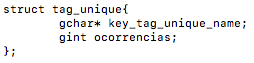
\includegraphics[scale=0.70]{image_tag_unique}
\caption{Estrutura \textit{Tag\_Unique}}
\label{img:tag_unique}
\end{figure}

\subsection{Clean}

Função que liberta a memória da \textbf{TCD\_community}. Por consequência,
realiza o \textbf{free} da estrutura \textbf{utilizador}, utilizando a 
função da \textit{glib}, \textbf{g\_hash\_table} \textbf{\_foreach}. 
De seguida, libertamos a própria \textit{\textbf{GHashTable*}} através da 
função \textbf{g\_hash\_table\_destroy}. O mesmo sucede-se com a estrutura
\textbf{posts} e \textbf{tag}. A estrutura \textbf{date\_posts}, sendo
uma \textit{\textbf{GList*}} tem uma forma diferente de libertar a 
memória. Para tal ser efetuado vamos a todos os parâmetros da mesma
e usamos a função \textbf{g\_list\_remove} para libertar a memória
de todos os elementos constituintes da lista em questão. De seguida,
realizamos o \textbf{g\_list\_free} de forma a libertar a própria 
estrutura.

\section{Conclusão}
\label{sec:conclusao}

Tendo em conta os objetivos definidos, o grupo acha que os resultados 
principais foram obtidos. Além de aprender a trabalhar com ficheiros 
do tipo \textbf{XML}, aprendemos a trabalhar com a biblioteca \textbf{GLib}.
Aliamos também uma evolução da nossa aprendizagem no tema do 
\textbf{encapsulamento}, da \textbf{modularidade} e 
da \textbf{abstração de dados}.

Outros objetivos alcançados são a resolução total das queries e a eficiência
que se faz notar nestas mesmas.

De uma forma natural, o grupo sentiu dificuldades durante o projeto, sendo 
uma, por exemplo, a necessidade de alterar a base total do trabalho devido
a termos inicialmente considerado a ordenação dos ficheiros, quando só nos
faltava resolver a query 11.

\section{Bibliografia}

\begin{enumerate} 
	\item Prof. F. Mário Martins, \textit{Programação Modular em C};
	\item Prof. F. Mário Martins, \textit{Tipos Incompletos em C}.
\end{enumerate}

\end{document}